
\chapter{Background}

\section{Immunology concepts}

\subsection{Our immune system} \label{bg:immunesystem}

Our immune system consists of organs, cells and groups of cells working in unison to defend us from outside organisms that could pose a danger to our health. Such outside forces could be harmful bacteria or parasites. The human body is a haven for these to thrive in, at our detriment. Our immune system protects us by attacking these foreign bodies – antigens – when they are detected and filed as dangerous. The key in this exchange is for our immune system to recognise which bodies are ours, and which are outsider, potentially dangerous forces (\cite{http://www.imgt.org/IMGTeducation/Tutorials/ImmuneSystem/UK/the_immune_system.pdf}).

\begin{figure}[h]
    \centering
    \begin{subfigure}[h!]{0.3\textwidth}
        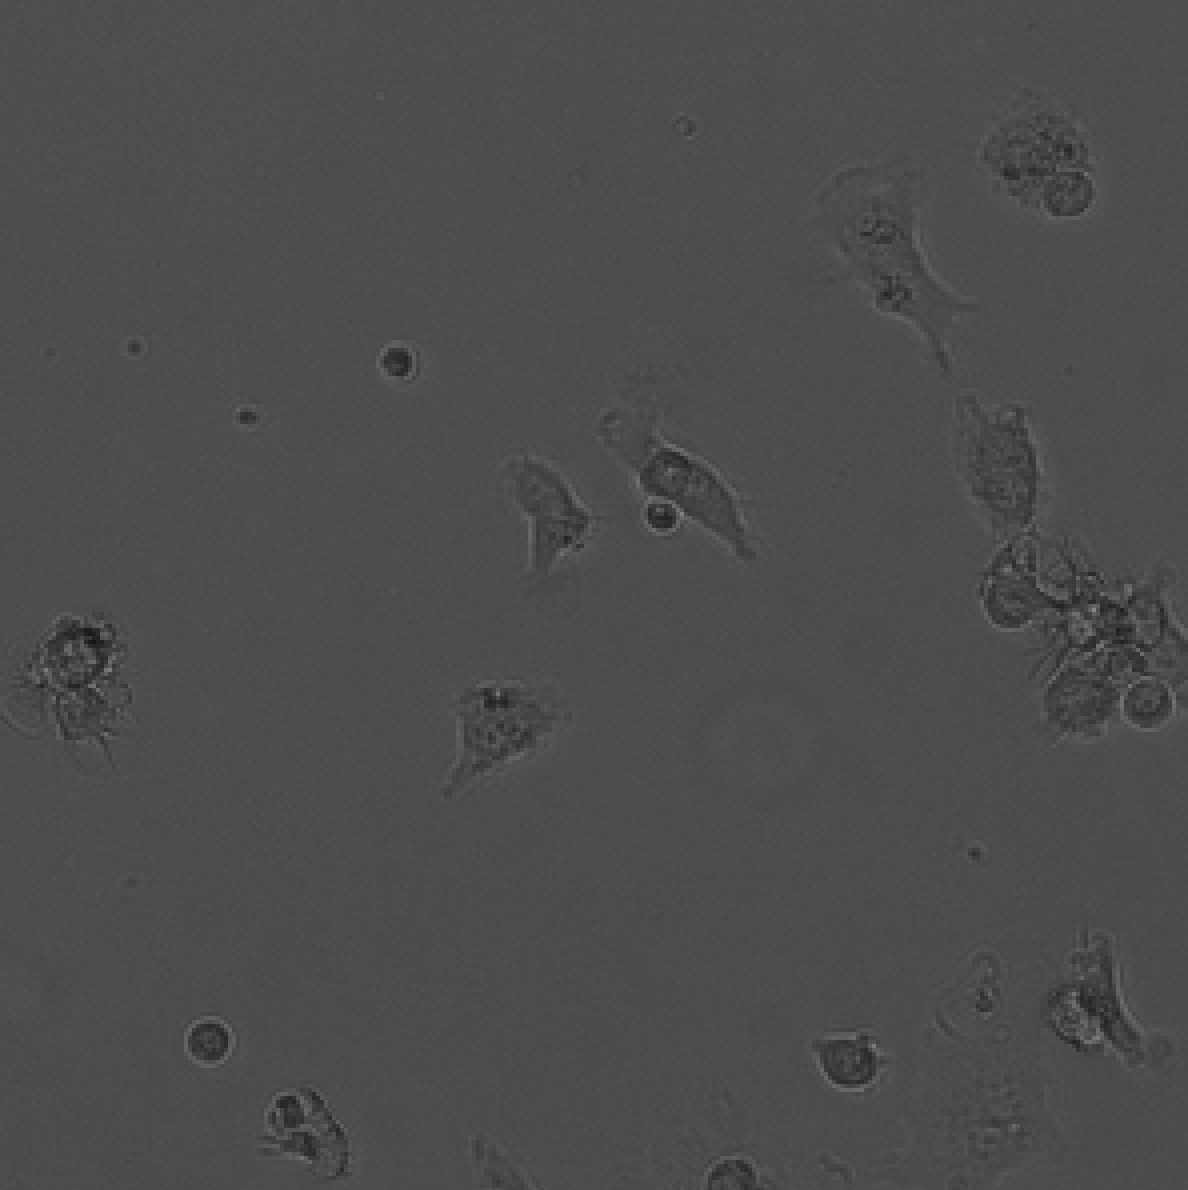
\includegraphics[width=\textwidth]{dissertation/figures/example_DCs.png}
    \end{subfigure}
    \begin{subfigure}[h!]{0.3\textwidth}
        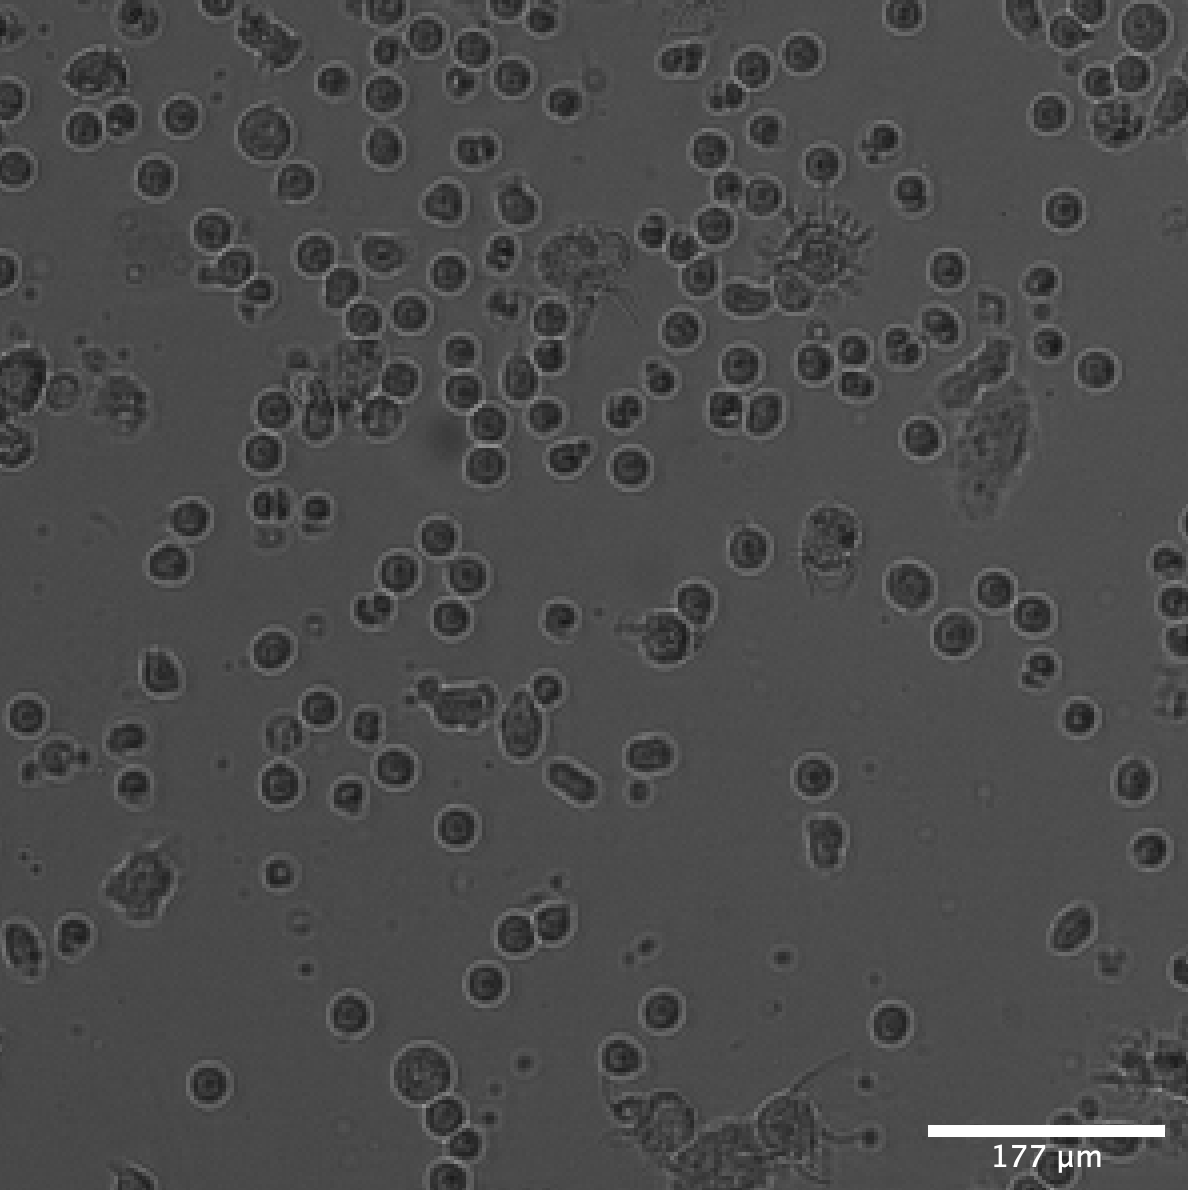
\includegraphics[width=\textwidth]{dissertation/figures/example_Tcells.png}
    \end{subfigure}
    \caption{Microscopic images of dendritic cells (left) and T cells (right) in an assay. Scale: , 200x zoom.}
\end{figure}

\begin{figure}[h]
    \centering
    \begin{subfigure}[h!]{0.3\textwidth}
        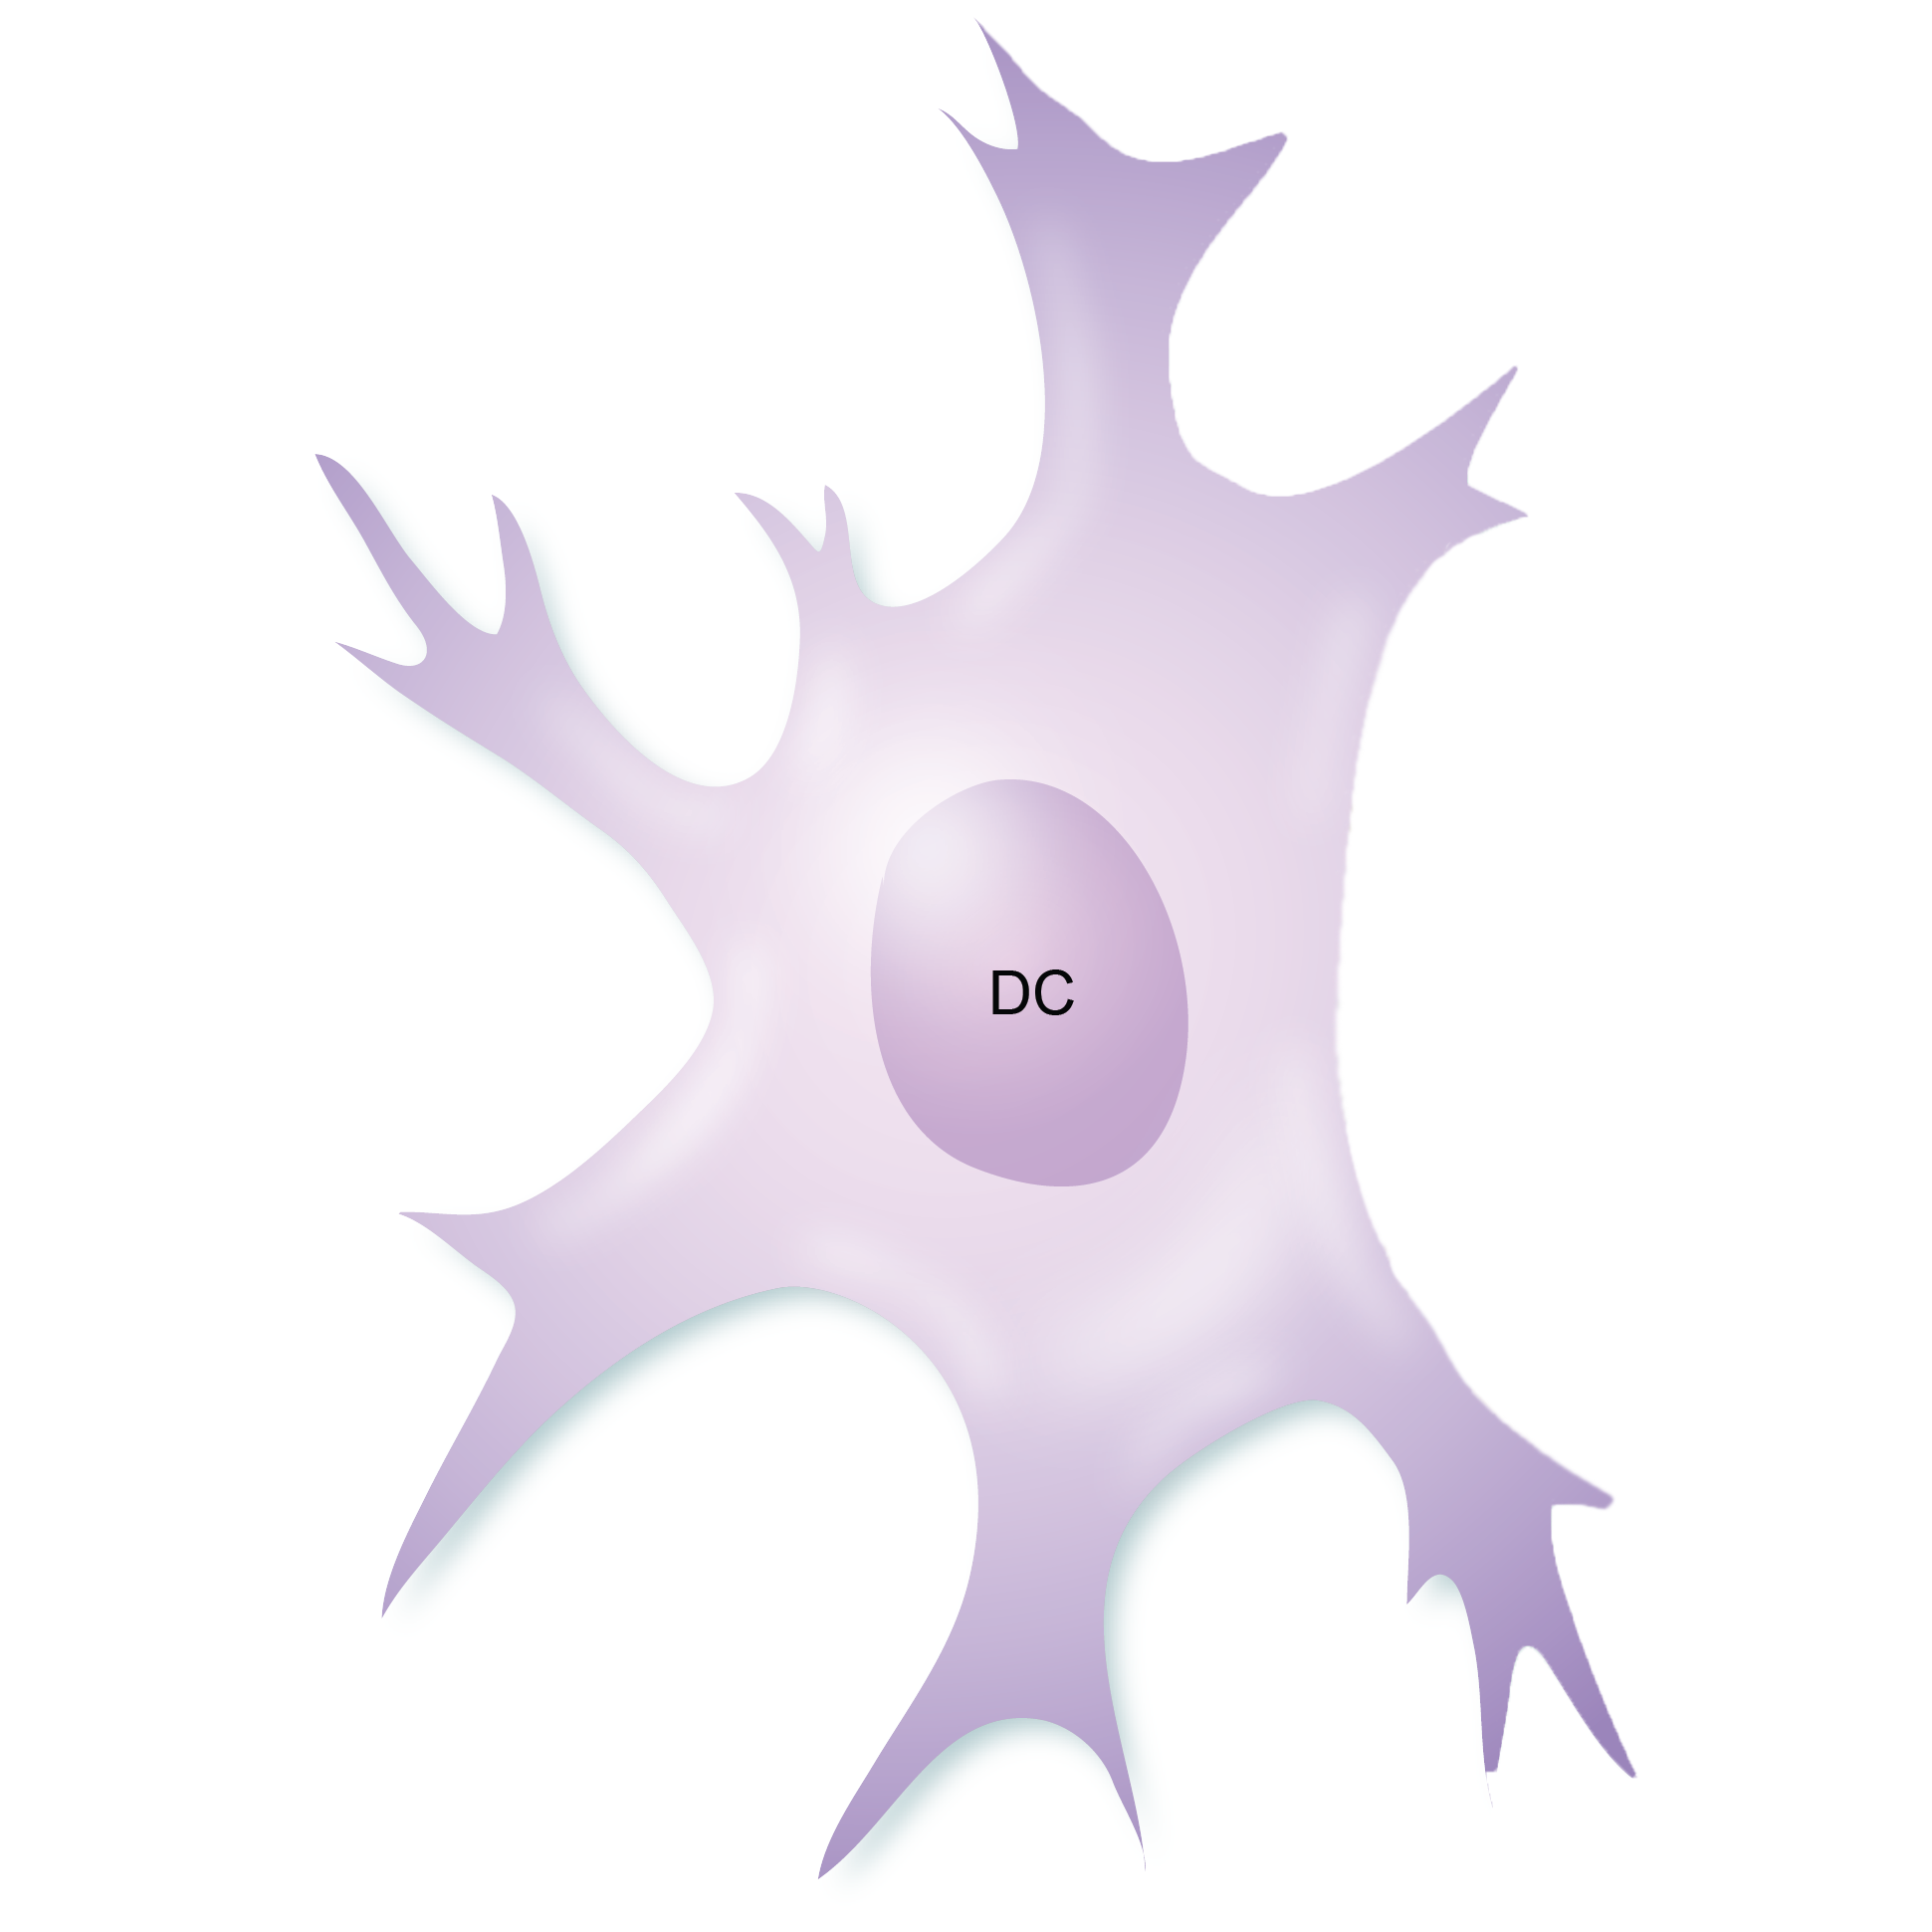
\includegraphics[width=\textwidth]{dissertation/figures/model_DC.png}
    \end{subfigure}
    \begin{subfigure}[h!]{0.3\textwidth}
        
\includegraphics[width=\textwidth]{dissertation/figures/model_Tcell.png}
    \end{subfigure}
    \caption{Model of a dendritic cell (left) and a T cell (right). Adapted from \cite{https://www.immunology.org/public-information/bitesized-immunology/systems-and-processes/t-cell-activation}}
    \label{eval:graphs}
\end{figure}

% What is the scale of the microscopic images?

The key defenders of our bodies are thus the actors of our immune systems. The actors we are interested in for the purpose of this research are T lymphocytes – "T cells" – and dendritic cells – DCs. Dendritic cells are "sentinels" and initiate our immune system's responses by processing their environment and sending the information over to T cells. T cells are "master controllers" and trigger the appropriate immune response, if any, from the information they have received from dendritic cells (\cite{https://www.immunology.org/public-information/bitesized-immunology/cells/dendritic-cells, https://www.youtube.com/watch?v=hRvyCYyab68}). [how to give more detail without losing reader? is this sufficient?]

%They interact with T cells, interactions which might be transient if nothing is to be triggered, or more communicative (\cite{https://www.youtube.com/watch?v=hRvyCYyab68}). 

%The idea is that we can stimulate this interaction between dendritic cells and T cells through different drug components, both for inhibition or increase of level of interaction. 

\subsection{Effects of interaction between immune cells} \label{bg:interaction}

Antigens, which is the encapsulating term for all threats to our immune system, can be fought by antibodies, which are defensive proteins produced by our immune system. More specifically, antibodies are produced by some immune cells in a process which starts in T cells, and in some cases is activated by T cells seeing antigens on the surface of dendritic cells (\cite{https://elifesciences.org/articles/06994}). Hence, the interaction between dendritic cells and T cells is critical in the decision for our immune system to produce agents to defend our body.

The purpose of this dissertation is to evaluate how much interaction is witnessed between immune cells. There is existing work in the field of immunology looking into the effects of these changes in interaction. Benson et al. show how the generation of antibodies might be impacted by T cell and dendritic cell interaction. They studied how dendritic cells and T cells interacted in mice's immune systems, both in terms of duration and whether or not interaction was indeed witnessed. This interaction was studied under different conditions, with different drug compounds being used to attempt to drive interaction or inhibit it. They found that in conditions where compounds were blocking interaction between T cells and DCs, less antibodies were generated, meaning that the mice were not defending themselves as much. Hence, the study of the impact of compounds on the interactions between immune cells can tell us how our immune system could react. 

\subsection{Implications}

Concepts and research highlighted in Sections \ref{bg:immunesystem} and \ref{bg:interaction} show that changes in interactions between immune cells control the way in which our immune system protects itself. Hence, analysing the interaction between immune cells under different experimental conditions poses a particular interest in the field of immunology for studying immune responses. We want to analyse this interaction with the help of deep learning techniques. 

% title: qualifying interaction
\section{Concepts of interest in Deep Learning}

The following sections collate selected research that show how deep learning techniques could be applied in our context of study. 

\subsection{Convolutional Neural Networks for image feature extraction}

%A number of approaches already use deep neural networks for classification from textual genome sequences, particularly for cancer type detection (\cite{https://www.biorxiv.org/content/10.1101/612762v1}, \cite{https://www.nature.com/articles/s41598-019-53989-3}). 
Convolutional operations in neural networks were first introduced by Fukushima at the start of the 1980s for pattern recognition. They were later popularised by LeCun as a method for object recognition, once back-propagation was put to use as a learning procedure for networks. LeCun applied his convolutional neural network to digit recognition and classification. Since then, convolutional operations in neural networks have proven to be successful to extract features from images. In a recent medical example, Shen et al. trained a convolutional neural network structure to detect breast cancer from mammography screenings and which showed competitive results compared to commercial systems (\cite{https://www.nature.com/articles/s41598-019-48995-4}). 
[how much research to cite in this context? there is a lot available]

\subsection{Autoencoders for dimensionality reduction}

An autoencoder is a type of neural network trained to map its input to its output from a compressed representation of the input, as shown in Figure \ref{fig:autoencoder}. The compressed representation of the input obtained from the bottleneck layer is a \textit{coded} representation of the input, while the final output of the network is the \textit{decoded} version of the input. Autoencoders are not trained to learn a perfect copy of the input data, but a smaller, compressed copy with features which the neural network learns to be most important to be able to gain and overall understanding of the input. Autoencoders were first introduced in the 1980s (LeCun, DE Rumelhart) and are traditionally used for dimensionality reduction and feature extraction (\cite{http://www.deeplearningbook.org/contents/autoencoders.html}). 

\begin{figure}[h!]
    \centering
    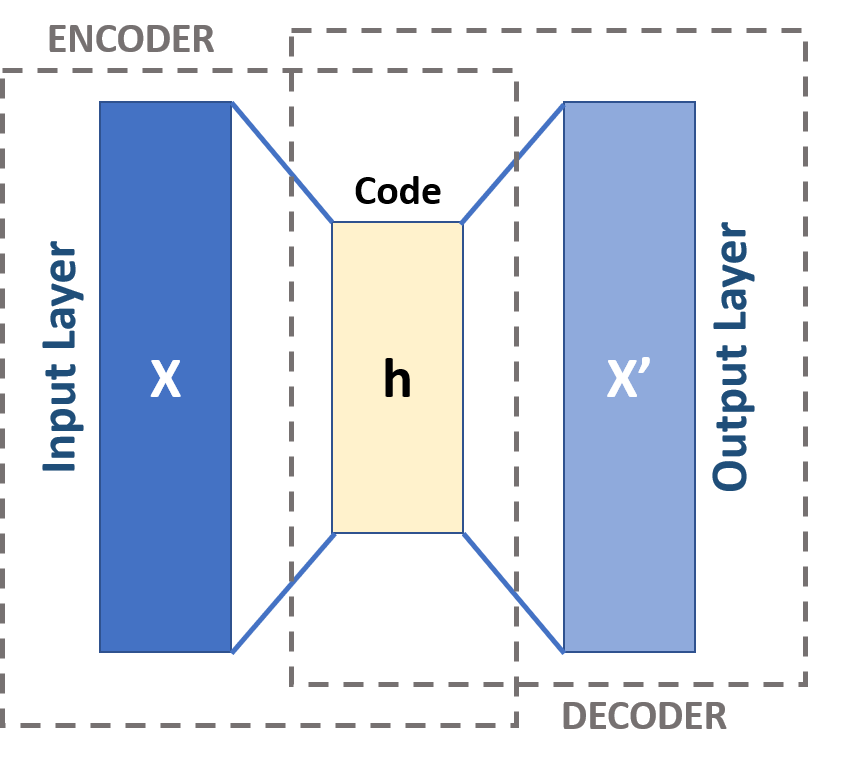
\includegraphics[width=0.45\textwidth]{dissertation/figures/autoencoder_schema.png}
    \caption{Autoencoder representation. To be recreated in Photoshop. Current source: Wikipedia}
    \label{fig:autoencoder}
\end{figure}

Zamparo and Zhang, 2015 (\cite{https://arxiv.org/pdf/1501.01348.pdf}) show that autoencoders can be successfully applied for dimensionality reduction in the context of biomedical data. Their autoencoder approach, applied to the unsupervised clustering of cell phenotypes, outperformed other dimensionality reduction techniques such as Principal Component Analysis (PCA). However, the context of this approach was not on imaging data. 

% http://arxiv.org/abs/1809.00027
Nonetheless, autoencoders have been successfully used for reducing the dimensionality of large imaging data by using convolution operations in their structure. Saenz et al. successfully used convolutional autoencoders for feature extraction from climate imaging data. %More famously, convolutional autoencoders have been shown to be efficient in improving the clustering of the MNIST dataset, when visualised with high-visualising techniques like t-sne and UMAP. t-sne and UMAP are of interest to us as they allow to project high-dimensional data onto 2 dimensions (or three in the case UMAP). Using them allows us to assess whether or not our data has some underlying structure – e.g. whether or not we can cluster cells according to different experimental conditions. 

\subsection{Deep regression models}

Deep neural networks can also be used to make real-valued prediction, rather than categorised. Moussavi-Khalkhali and Jamshidi used autoencoders trained with Stochastic Gradient Descent to predict timeseries data \cite{https://ieeexplore.ieee.org/document/7838202}. 

\section{Finding structure in high-dimensional data}

The data we are studying consists of images of cells obtained through high content screening (HCS). HCS is a method for capturing images of cells in multi-well plates, using high-resolution microscopy \cite{https://www.ncbi.nlm.nih.gov/pubmed/23035272}. A plate captured with high content screening can yield a large number of images in very high-resolution, e.g. 2048x2048 pixels. This makes the analysis of the physical characteristics of a cell possible at a granular level. However, it could be of interest to us to gain an understanding of the overall structure of the data, in which case the high dimensionality of each data point (each image) will be harder. 

The following sections highlight available techniques that can be used to look for structure in a group of high-dimensional data points.

%High content screening (HCS) is a method for capturing images of cells in multi-well plates, using high-resolution microscopy. It can be used to analyse physical characteristics of the cells captured on images. HCS is a choice method for analysing how compounds can alter cells from images, i.e. drug discovery \cite{https://www.ncbi.nlm.nih.gov/pubmed/23035272}. 

\subsection{t-SNE}
t-distributed stochastic neighbor embedding (t-SNE) was developed in 2008 by van der Maaten and Hinton as a technique to map high-dimensional data to a two- or three-dimensional space. t-SNE can find structure in high-dimensional data points by using the local relationships between data points and optimising results using gradient descent. [how much detail to go into? don't want to go off tangent]%These local relationships are defined using a Gaussian probability distribution in high dimensional space, and then recreated using the Studnet t-distribution. 

\subsection{UMAP}
Uniform Manifold Approximation and Projection for Dimension Reduction (UMAP) is a dimensionality reduction technique which was published in 2018 and has shown competitive results compared to t-SNE. 

\section{The place of Deep Learning in immunology}

There is a number of existing research that use broader machine learning techniques in the field of immunology. Muh et al (\cite{https://www.ncbi.nlm.nih.gov/pubmed/19516900/} applied Support Vector Machines (SVMs) to the study of allerginicity. Allergic reactions are triggered when a immune system wrongly triggers an immune response and produces antibodies to attack a normally harmless substance, such as dust (\cite{https://www.immunology.org/policy-and-public-affairs/briefings-and-position-statements/allergy}). The SVMs were used to analyse the DNA sequences of known allergens and known non-allergens. The aim was to try and make accurate predictions on unseen sequences and classify them as either allergenic or non-allergenic. The model achieved 95.3\% accuracy. %Similarly, MP et al. \cite{https://www.ncbi.nlm.nih.gov/pubmed/20144194/} used a Bayesian classifier and a decision tree to predict the likelihood of degenerative disorders from the sequencing of antibodies. 

[other example here]

\bigskip 
This section has demonstrated that immunology-related fields such as cancer detection have successfully applied deep learning methods in their research to obtain promising results, and that immunology researchers have also successfully made use of machine learning techniques. [CONFIRM: Furthermore, deep learning has been applied in immunology for sequencing based analysis, (as well as cell segmentation?).] The research cited here highlights that there is an array of methods available to process high-dimensional, visual data and analyse it with the help of deep learning. However, there seems to be a lack of research into the qualitative and quantitative analysis of immune cell interactions from imaging data through these techniques. This paper will thus focus on filling this gap by using deep learning to extract features from images of cells in order to uncover qualitative or quantitative data about the interactions between types of immune cells. [INTRODUCTION?: Subsequently, the results of this research could show whether this shows promise and should be explored further in the future.]